\subsection{Programmablauf} % Johannes


\subsection{Partitionierung des Codes} % Flo
\begin{frame}
	\frametitle{Partitionierung des Codes}
	\framesubtitle{Grundlagen}
	\textbf{Ziel:} Finden von sinnvollen Übersetzungseinheiten
	
	\vspace{0.50cm}
	
	\textbf{Überlegung:}
	\begin{itemize}
		\item einzelne Instruktionen übersetzen zu aufwändig
		\item keine Übersetzung des ganzen Programmes
		\item[\conclude] Übersetzung von \textit{Basic Blocks}
	\end{itemize}
	
	\vspace{0.50cm}
	
	\begin{block}{Definition: Basic Block}
		\begin{itemize}
			\item einziger Ein- und Ausgangspunkt
			\item enthaltene Instruktionen der Reihe nach ausgeführt
		\end{itemize}
	\end{block}
\end{frame}

\begin{frame}
	\frametitle{Partitionierung des Codes}
	\framesubtitle{Finden von Blockgrenzen}
	
	\textbf{Blockende} durch folgende Instruktionen erreicht:
	\begin{itemize}
		\item Unbedingte Sprünge \& Funktionsaufrufe (\texttt{j}, \texttt{call}, \texttt{ret}) % todo I'll list the pseudos here, if that's fine?
		\item Bedingte Sprünge (\texttt{beq}, \texttt{bne}, \texttt{blt}, \texttt{bge}, \texttt{bltu}, \texttt{bgeu})
		\item System Calls (\texttt{ecall})
	\end{itemize}
	
	\vspace{0.50cm}
	
	\textbf{Optimierungspotenzial:}
	\begin{itemize}
		\item Sprüngen folgen
		\item rekursive Übersetzung von Sprungzielen
		\item Schwierigkeiten bei bedingten Sprüngen
	\end{itemize}
	
\end{frame}

\begin{frame}
	\frametitle{Partitionierung des Codes}
	\framesubtitle{Beispiel}

	\textbf{\color{blue} Sprungverfolgung} zu \texttt{\color{blue} label},\\
	\textbf{\color{red} Blockende} durch \texttt{\color{red}ecall}.

	\vspace{1.5cm}
	
	\begin{columns}[onlytextwidth]
		\ttfamily
		\begin{column}{0.49\textwidth}
			add  x6, x6, x7\\
			slli x6, x6, 3\\
			xori x7, x7, -1\\
			{\color{blue} j label}
		\end{column}
		
		\begin{column}{0.49\textwidth}
			{\color{blue} label:}\\
			addi a0, x0, 0\\
			addi a7, x0, \_\_NR\_exit\\
			{\color{red} ecall}
		\end{column}
	\end{columns}
\end{frame}


\subsection{Codegenerierung und Cache} % Flo
\begin{frame}
	\frametitle{Codegenerierung}
	\framesubtitle{Grundlagen}
	\textbf{Ziel:} Generieren von äquivalentem Code
	
	\vspace{0.50cm}
	
	\textbf{Prinzipieller Ansatz:} Instruktions-Mapping x86--64 \conclude RISC--V
	
	\begin{itemize}
		\item Übersetzungen jeder Instruktion der Quellarchitektur
		\item Probleme durch architektonische Unterschiede
		\begin{itemize}
			\item \textit{load-store}- vs. \textit{register-memory-Architektur}
			\item \textit{Zwei}- bzw. \textit{Dreiadressform}
		\end{itemize}
		
		\item Mustererkennung im Eingangscode
	\end{itemize}
\end{frame}

\begin{frame}
	\frametitle{Codegenerierung}
	\framesubtitle{Beispiel: Architektonische Unterschiede}
	
	\textbf{Problem:} ein Operand ist implizites Zielregister (x86)
	
	\vspace{2cm}
	
	\begin{columns}[onlytextwidth]
		\ttfamily
		\begin{column}{0.45\textwidth}
			\centering
			sub rd, rs1, rs2
		\end{column}
		
		\begin{column}{0.05\textwidth}
			\centering
			\conclude
		\end{column}
		
		\begin{column}{0.45\textwidth}
			\centering
			mov rd, rs1\\
			sub rd, rs2
		\end{column}
	\end{columns}
\end{frame}


\begin{frame}
	\frametitle{Codegenerierung}
	\framesubtitle{Beispiel: Optimierte Übersetzung}
	
	\textbf{Optimierungsmöglichkeit:} äquivalente native Instruktion existiert
	
	\vspace{2cm}
	
	\begin{columns}[onlytextwidth]
		\ttfamily
		\begin{column}{0.45\textwidth}
			\centering
			xori rd, rd, -1
		\end{column}
		
		\begin{column}{0.05\textwidth}
			\centering
			\conclude
		\end{column}
		
		\begin{column}{0.45\textwidth}
			\centering
			not rd
		\end{column}
	\end{columns}
\end{frame}


\begin{frame}
	\frametitle{Codegenerierung}
	\framesubtitle{Beispiel: Macro Operation Fusion}
	
	\textbf{Optimierungsmöglichkeit:} mehrere Instruktionen bündeln
	
	\vspace{2cm}
	
	\begin{columns}[onlytextwidth]
		\ttfamily
		\begin{column}{0.45\textwidth}
			\centering
			lui rd, imm1\\
			addi rd, rd, imm2
		\end{column}
		
		\begin{column}{0.05\textwidth}
			\centering
			\conclude
		\end{column}
		
		\begin{column}{0.45\textwidth}
			\centering
			mov rd, (imm1 + imm2)
		\end{column}
	\end{columns}
\end{frame}


\begin{frame}
	\frametitle{Code Cache}
	\framesubtitle{Konzept}
	
	\textbf{Hintergrund:} Angetroffene Basic Blocks sollen nur ein Mal übersetzt werden.
	
	\vspace{0.50cm}
	
	\begin{block}{Code Cache}
		\begin{itemize}
			\item Speicherregion, in die generierter Code geschrieben wird
			\item Index für die Speicherregion für schnellen Lookup (\refer Hash-Tabelle, TLB)
		\end{itemize}
	\end{block}
	
	\vspace{0.50cm}
	
	\textbf{Nutzung:}
	
	\begin{itemize}
		\item Block wird nach erstem Übersetzen in den Cache geschrieben
		\item Lookup vollzieht Adressübersetzung RISC--V \refer x86
		\item kein Löschen von übersetzten Blöcken (\refer Optimierungen)
	\end{itemize}
\end{frame}


\begin{frame}[c]
	\frametitle{Code Cache}
	\framesubtitle{Programmfluss (vereinfacht)}
	\centering
	\begin{figure}
		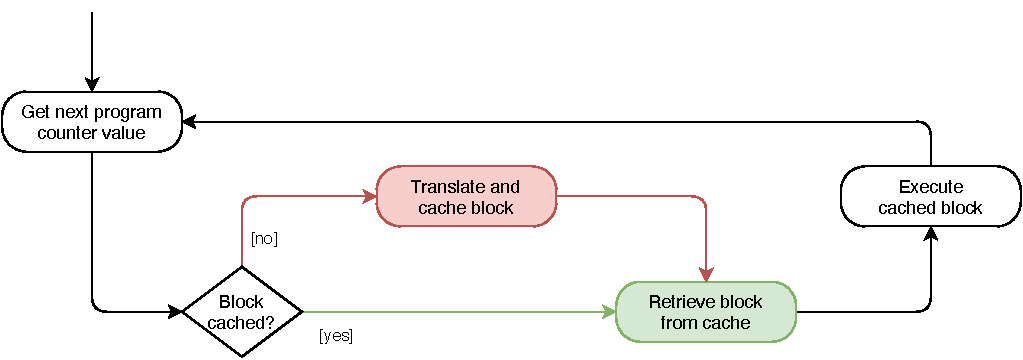
\includegraphics[width=\textwidth]{diagrams/cache-flow}
	\end{figure}
\end{frame}


\subsection{Registernutzung} % Flo


\subsection{Optimierungen} % Johannes

